\section{The universal enveloping algebra}
The following hold for this section alone: We fix an arbitrary field $k$ and a Lie algebra $\g$ over $k$. By a $k$-algebras we always mean an associative and unitary one, and homomorphisms of $k$-algebras have to respect the unit.





\subsection{Definition, properties and construction}


\begin{defi}
 An \emph{universal enveloping algebra} of $\g$ is an $k$-algebra $\Ue(\g)$ together with a homomorphism of Lie algebras $\iota \colon \g \to \Ue(\g)$ such that for every $k$-Algebra $A$ and homomorphism of Lie algebras $\phi \colon \g \to A$ there exists a unique homomorphism of $k$-algebras $\Phi \colon \Ue(\g) \to A$ with $\phi = \Phi \circ \iota$, i.e.\ making the following diagram commute:
 \begin{center}
  \tikzsetnextfilename{universal_property_of_universal_enveloping_algebra}
  \begin{tikzpicture}[node distance = 5em]
   \node (g) {$\g$};
   \node[below of = g] (Ug) {$\Ue(\g)$};
   \node[right = 5em of Ug] (A) {$A$};
   \draw[->] (g) to node[left] {$\iota$} (Ug);
   \draw[->] (g) to node[above right] {$\phi$} (A);
   \draw[->, dashed] (Ug) to node[below] {$\Phi$} (A);
  \end{tikzpicture}
 \end{center}
\end{defi}


\begin{rem}
 As always with universal objects any two enveloping algebras of $\Ue(\g)_1$ with $\iota_1 \colon \g_1 \to \Ue(\g)_1$ and $\Ue(\g)_2$ with $\iota_2 \colon \g \to \Ue(\g)_2$ of $\g$ are isomorphic, and there exists a unique isomorphism $\varphi \colon \Ue(\g_1) \to \Ue(\g_2)$ with $\iota_2 = \varphi \colon \iota_1$, i.e.\ making the following diagram commute:
 \begin{center}
  \tikzsetnextfilename{uniqueness_of_universal_enveloping_algebra}
  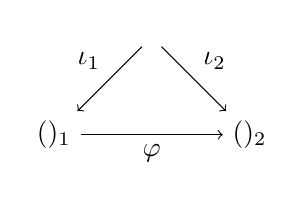
\begin{tikzpicture}[node distance = 5em]
   \node (g) {$\g$};
   \node[below left of = g] (U1) {$\Ue(\g)_1$};
   \node[below right of = g] (U2) {$\Ue(\g)_2$};
   \draw[->] (g) to node[above left] {$\iota_1$} (U1);
   \draw[->] (g) to node[above right] {$\iota_2$} (U2);
   \draw[->] (U1) to node[below] {$\varphi$} (U2);
  \end{tikzpicture}
 \end{center}
 Hence we will talk about \emph{the} universal enveloping algebra of $\g$.
\end{rem}


\begin{lem}
 Let $T(\g) = \bigoplus_{n=0}^\infty \g^{\otimes n}$ be the tensor algebra and $\mc{I} \subseteq T(\g)$ the two-sided ideal generated by the element $x \otimes y - y \otimes x - [x,y]$ with $x,y \in \g$. The the quotient $\Ue(\g) \coloneqq T(\g)/\mc{I}$ together with the $k$-linear map
 \[
  \iota \colon \g \to \Ue(\g), \quad x \mapsto x + \mc{I}
 \]
 is an universal enveloping algebra of $\g$.
\end{lem}
\begin{proof}
 $\Ue(\g)$ is a $k$-algebra by construction and $\iota$ is a homomorphism of Lie algebras since for all $x,y \in \g$
 \begin{align*}
  [\iota(x),\iota(y)]
  &= [x + \mc{I}, y + \mc{I}]
  = (x + \mc{I})(y + \mc{I}) - (y + \mc{I})(x + \mc{I}) \\
  &= (x \otimes y - y \otimes x) + \mc{I}
  = [x,y] + \mc{I}
  = \iota([x,y]).
 \end{align*}
 Given any $k$-algebra $A$ and homomorphism of Lie algebras $\phi \colon \g \to A$ it can be uniquely extended to a homomorphism of $k$-algebras $\hat{\phi} \colon T(\g) \to A$ via
 \[
  \hat{\phi}(x_1 \otimes \dotsb \otimes x_n) = \phi(x_1) \dotsm \phi(x_n)
  \quad \text{for all $n \geq 0$ and $x_1, \dotsc, x_n \in \g$}.
 \]
 Because $\phi$ is not only $k$-linear but even a homomorphism of Lie algebras it follows that for all $x,y \in \g$
 \[
  \hat{\phi}(x \otimes y - y \otimes x)
  = \phi(x)\phi(y) - \phi(y)\phi(x)
  = [\phi(x),\phi(y)]
  = \phi([x,y])
  = \hat{\phi}([x,y])
 \]
 It follows that $\hat{\phi}(x) = 0$ for every $x \in \mc{I}$. Hence $\hat{\phi}$ factors through a unique homomorphism of $k$-algebras
 \[
  \Phi \colon \mc{U}(\g) \to A, \quad
  x_1 \otimes \dotsb \otimes x_n + \mc{I} \mapsto \phi(x_1) \dotsm \phi(x_n)
 \]
 for all $n \geq 0$ and $x_1, \dotsc, x_n \in \g$. For every $x \in \g$ it follows that
 \[
  (\Phi \circ \iota)(x)
  = \Phi(\iota(x))
  = \Phi(x + \mc{I}) 
  = \phi(x),
 \]
 which is why $\phi = \Phi \circ \iota$. That $\Phi$ is the unique homomorphism of $k$-algebras with this properties follows from the uniqueness of $\hat{\phi}$.
\end{proof}


\begin{cor}
 The homomorphism $\iota \colon \g \to \Ue(\g)$ is injective. As a $k$-algebra $\Ue(\g)$ is generated by $\g$.
\end{cor}


\begin{rem}
 We will always identify $\g$ with its image under $\iota$.
\end{rem}





\subsection{Casimir elements}
For this subsection we additionaly assume that $\g$ is finite-dimensional. We also fix some bilinear form $\beta \colon \g \times \g \to k$ which is associative and non-degenerate.


\begin{defi}\label{defi: definition of Casimir element}
 Let $\varphi_1 \colon \g \otimes \g^* \to \End_k(\g)$ and $\varphi_2 \colon \g \to \g^*$ be the isomorphisms of vector spaces defined by
 \[
  \varphi_1(x \otimes \phi)(y) = \phi(y) x
  \quad\text{and}\quad
  \varphi_2(x) = \beta(x, \cdot)
  \quad\text{for all $x,y \in \g$ and $\phi \in \g^*$}.
 \]
 Then the image of $1$ under the map
 \begin{equation}\label{eqn: Casimir without coordinates}
  k
  \xrightarrow{\lambda \mapsto \lambda \id_\g}
  \End_k(\g)
  \xrightarrow{\varphi_1^{-1}}
  \g \otimes \g^*
  \xrightarrow{\id_\g \otimes \varphi_2^{-1}}
  \g \otimes \g
  \xrightarrow{x \otimes y \mapsto x y}
  \Ue(\g)
 \end{equation}
 is called the \emph{Casimir element of $\beta$} and denoted by $C_\beta$.
\end{defi}


\begin{lem}
 The Casimir element $C_\beta$ in central in $\Ue(\g)$, i.e.\
 \[
  x C_\beta = C_\beta x \quad \text{for every $x \in \Ue(g)$}.
 \]
\end{lem}
\begin{proof}
 Let $\varphi_1$ and $\varphi_2$ as in Definition \ref{defi: definition of Casimir element}.
 
 Because $\Ue(\g)$ is generated by $\g$ as a $k$-algebra it sufficies to show $C_\beta$ commutes with every $x \in \g$. Hence it is to show that
 \[
  [x,C_\beta] = 0 \quad \text{for every $x \in \g$},
 \]
 where $[\cdot,\cdot]$ denotes the Lie bracket in $\Ue(\g)$. To see this notice that in \eqref{eqn: Casimir without coordinates} every map is a homomorphism of representations of $\g$, where $\g$ acts trivially on $k$, i.e. $x.\lambda = 0$ for every $x \in \g$ and $\lambda \in \g$.
 
 That the first map $k \to \End_k(\g)$ is a homomorphism of representations follows from the fact that $\g$ acts trivially on $k$ and also trivially on the one-dimensional subspace $k \id_\g \subseteq \End_k(\g)$.
 
 That $\varphi_1$ is an isomorphism of representations is known from Propositon \ref{prop: list of homomorphism of representations}.
 
 That the third map $\g \otimes \g^* \to \g \otimes \g$ is a homomorphism of representations follows from Proposition \ref{prop: list of homomorphism of representations}, because the identity $\id_\g$ is a homomorphism of representations and and the isomorphism $\varphi_2$ is one by the associativity of $\beta$, as seen in Lemma \ref{lem: associative bilinear form induces homomorphism of representations}.
 
 That the fourth map $\psi \colon \g \otimes \g \to \Ue(\g), x \otimes y \mapsto xy$ is a homomorphism of representations follows from direct calculation, because for all $x,y,z \in \g$
 \begin{align*}
  \psi(x.(y \otimes z))
  &= \psi((x.y) \otimes z + y \otimes (x.z))
  = (x.y)z + y(x.z) \\
  &= [x,y]z + y[x,z]
  = xyz - yxz + yxz - yzx
  = xyz - yzx \\
  &= [x,yz]
  = x.(yz)
  = x.\psi(y \otimes z).
 \end{align*}
 
 Because every map in \eqref{eqn: Casimir without coordinates} is a homomorphism of representations it follows that their composition $\phi \colon k \to \Ue(\g)$ is also a homomorphism of representations. Definition \ref{defi: definition of Casimir element} is then equivalent to $\phi(1) = C_\beta$. Because $\g$ acts trivially on $k$ and $\phi$ is a homomorphism of representations it follows that $\g$ also acts trivially on the span of $C_\beta$. In particular
 \[
  0 = x.C_\beta = [x,C_\beta] \quad \text{for every $x \in \g$}.
  \qedhere
 \]
\end{proof}


\begin{lem}[Casimir in coordinates]
 Let $x_1, \dotsc, x_n$ be a basis of $\g$ and $x^1, \dotsc, x^n$ the dual basis of $\g$ with respect to $\beta$, i.e.\ $\beta(x_i, x^j) = \delta_{ij}$ for all $i,j = 1, \dotsc, n$. Then
 \[
  C_\beta = \sum_{i=1}^n x_i x^i.
 \]
\end{lem}
\begin{proof}
 Let $\varphi_1$ and $\varphi_2$ as in Definition~\ref{defi: definition of Casimir element}. In \eqref{eqn: Casimir without coordinates} $1$ is mapped to $\id_\g$, which is then mapped to $\sum_{i=1}^n x_i \otimes x_i^*$, where $x_1^*, \dotsc, x_n^*$ denotes the dual basis of $\g^*$. As $\varphi_2(x^i) = x_i^*$ it follows that $\sum_{i=1}^n x_i \otimes x_i^*$ is then mapped to $\sum_{i=1}^n x_i \otimes x^i$, which is then further mapped to the element $\sum_{i=1}^n x_i x^i$ in $\Ue(\g)$.
\end{proof}















